\section{Fase 4: Análisis Exploratorio de datos oncológicos}

En esta fase, el científico obtiene el conjunto de datos o imágenes que fueron organizados previamente por el ingeniero y realiza un \textit{Análisis exploratorio de datos} para descubrir patrones generales en la información generada. Cabe resaltar, que en esta fase el acompañamiento del medico experto en oncología es de vital importancia, ya que los datos o imágenes que van ser explorados por el científico pueden contener variables que pueden tener o no un valor significativo para el experto, ayudando así a determinar si el análisis planteado para responder la pregunta va o no por un buen camino, de modo que es posible que se agreguen o eliminen diversas variables para lograr el resultado esperado. Adicionalmente, es necesario que los diversos análisis generados estén apoyados con gráficas que sean entendibles por todo el \textit{Data Analysis Team}, esto con el proposito de aportar ideas, y desde esta fase ir encontrando posibles correlaciones entre las variables oncológicas.

\newpage
\begin{figure}
	\caption{Distribuciones del conjunto de datos del Carcinoma invasivo de mama (TCGA, Cell 2015).}\label{fig:foobar}
	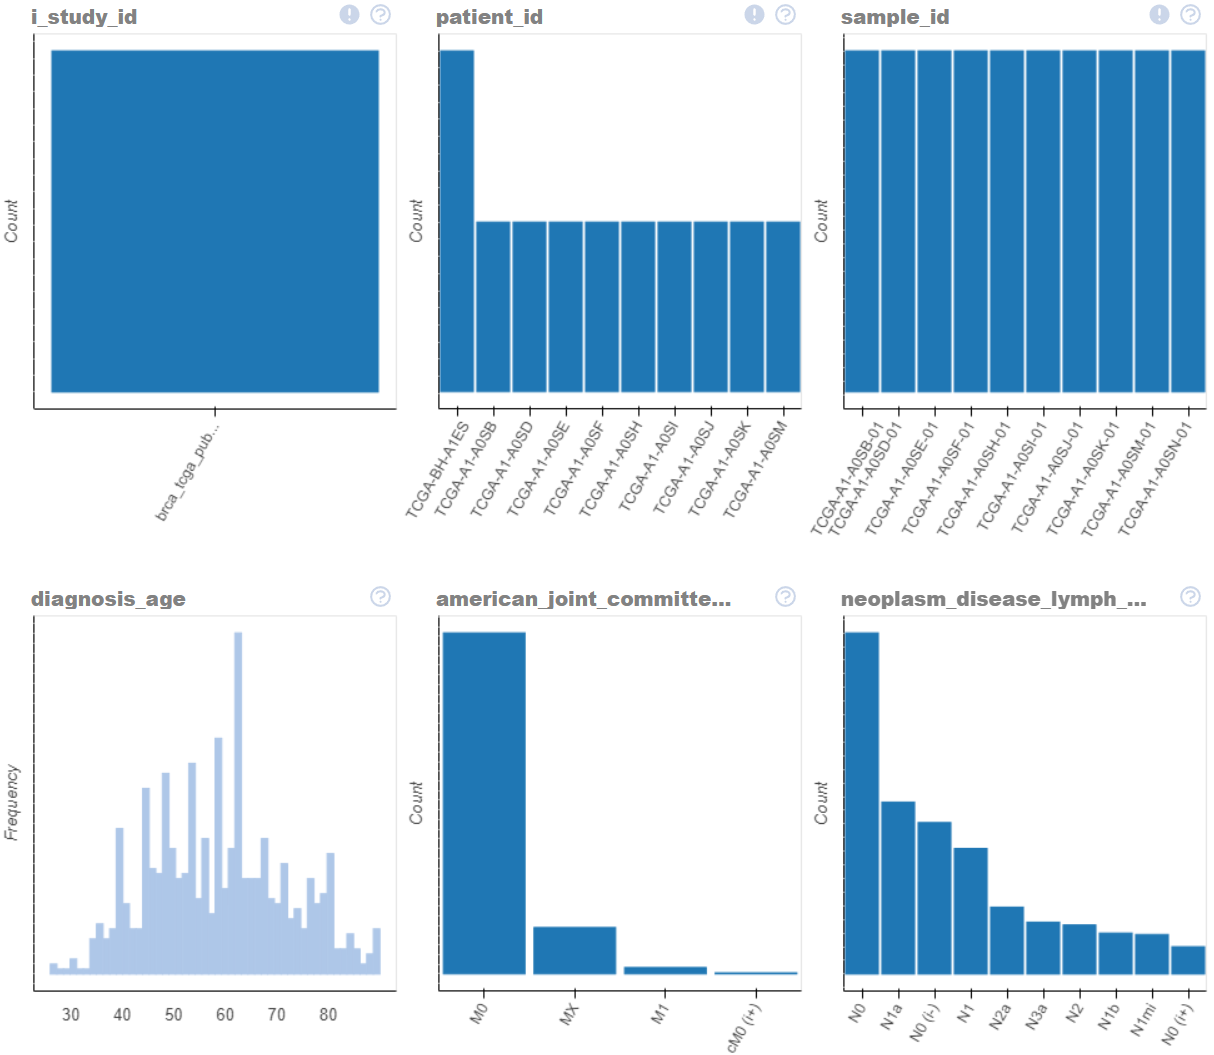
\includegraphics[width=0.9\textwidth]{NOTEBOOK/IMAGES_EDA/1}
	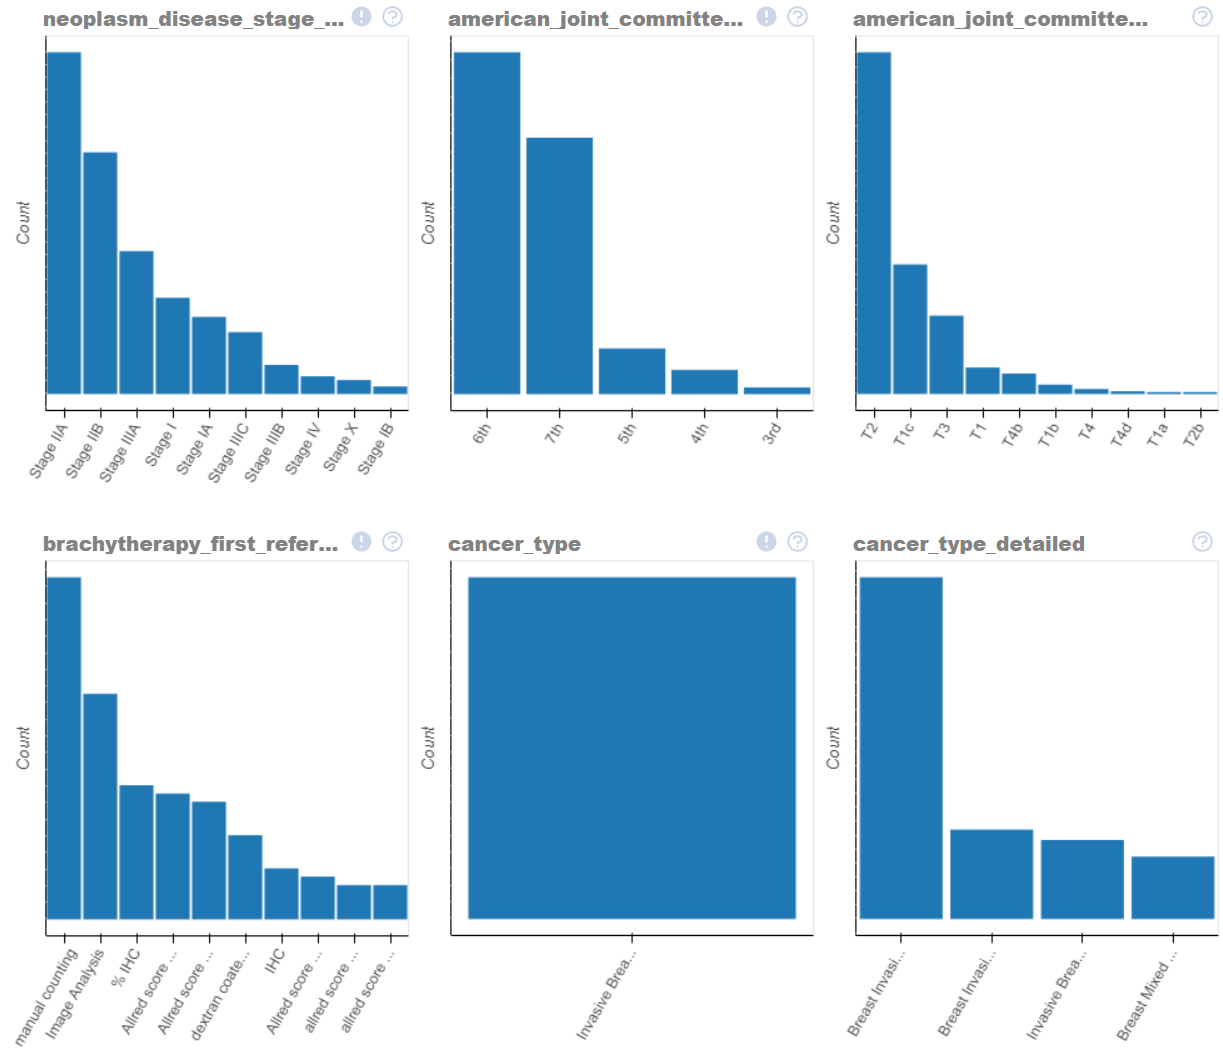
\includegraphics[width=0.9\textwidth]{NOTEBOOK/IMAGES_EDA/2}
\end{figure}

\begin{figure}
	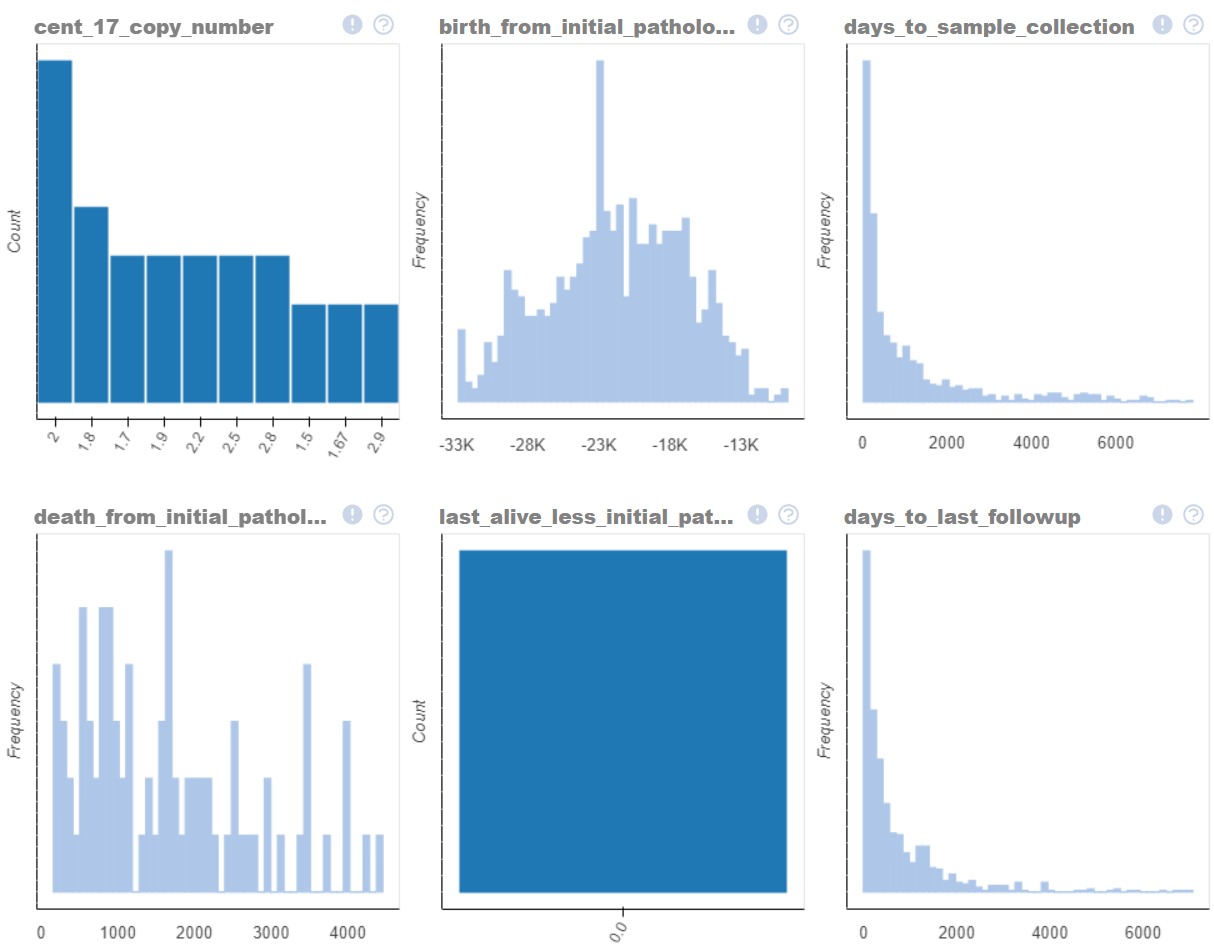
\includegraphics[width=0.9\textwidth]{NOTEBOOK/IMAGES_EDA/3}
	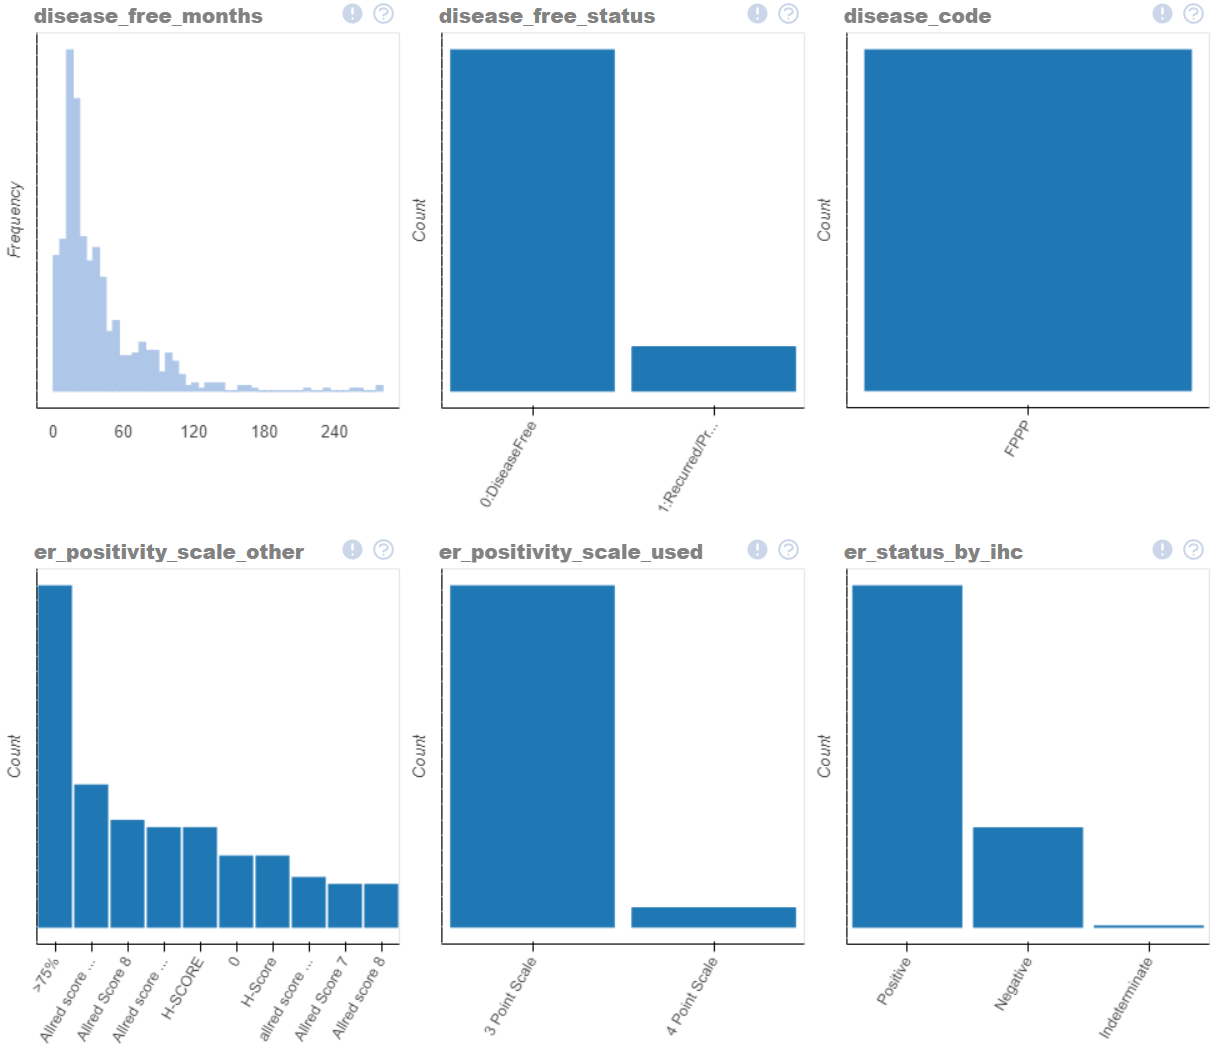
\includegraphics[width=0.9\textwidth]{NOTEBOOK/IMAGES_EDA/4}
\end{figure}

\begin{figure}
	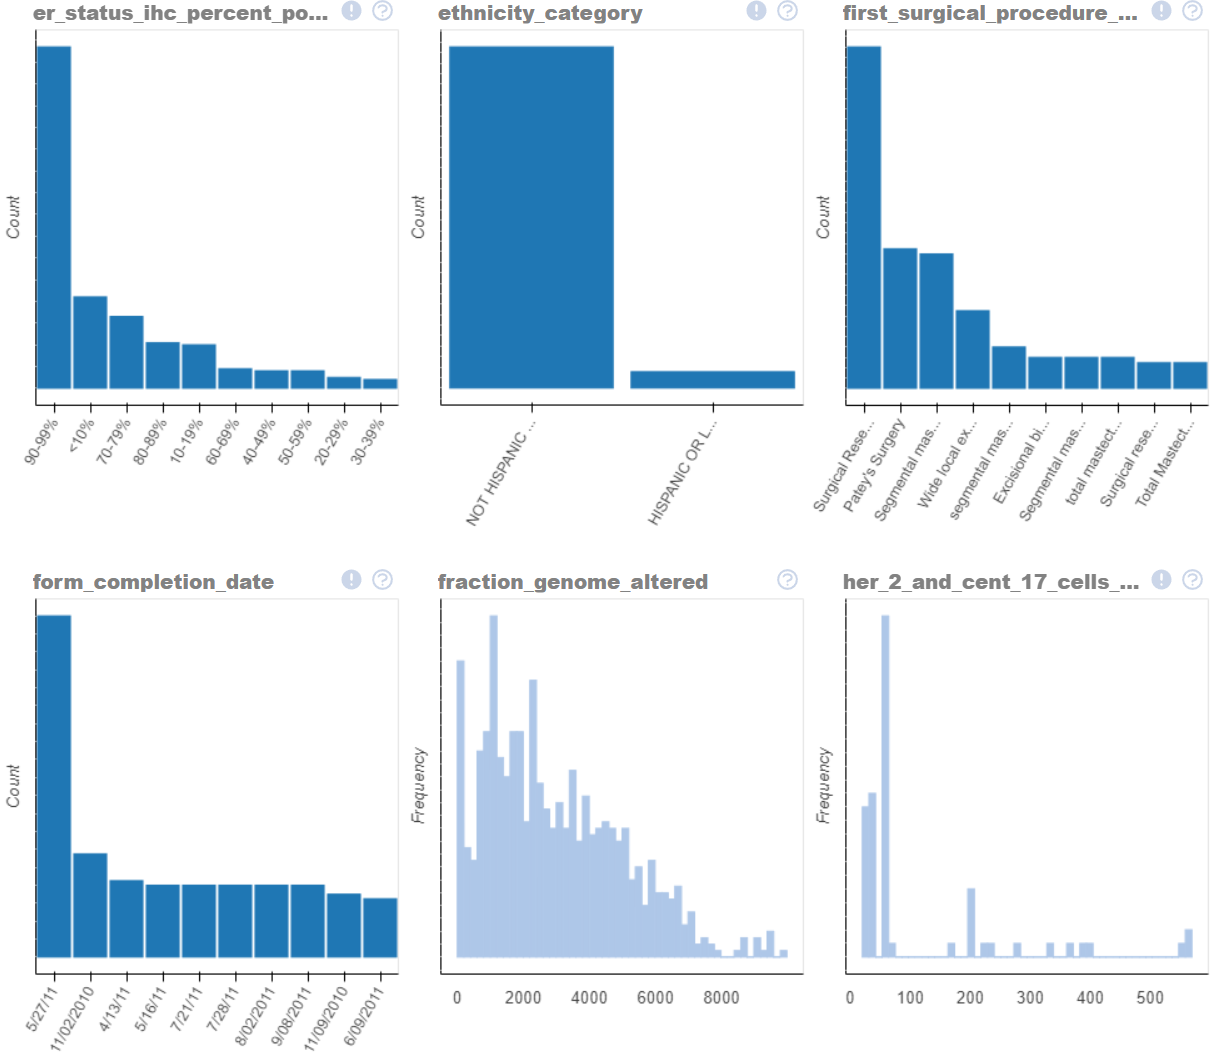
\includegraphics[width=0.9\textwidth]{NOTEBOOK/IMAGES_EDA/5}
	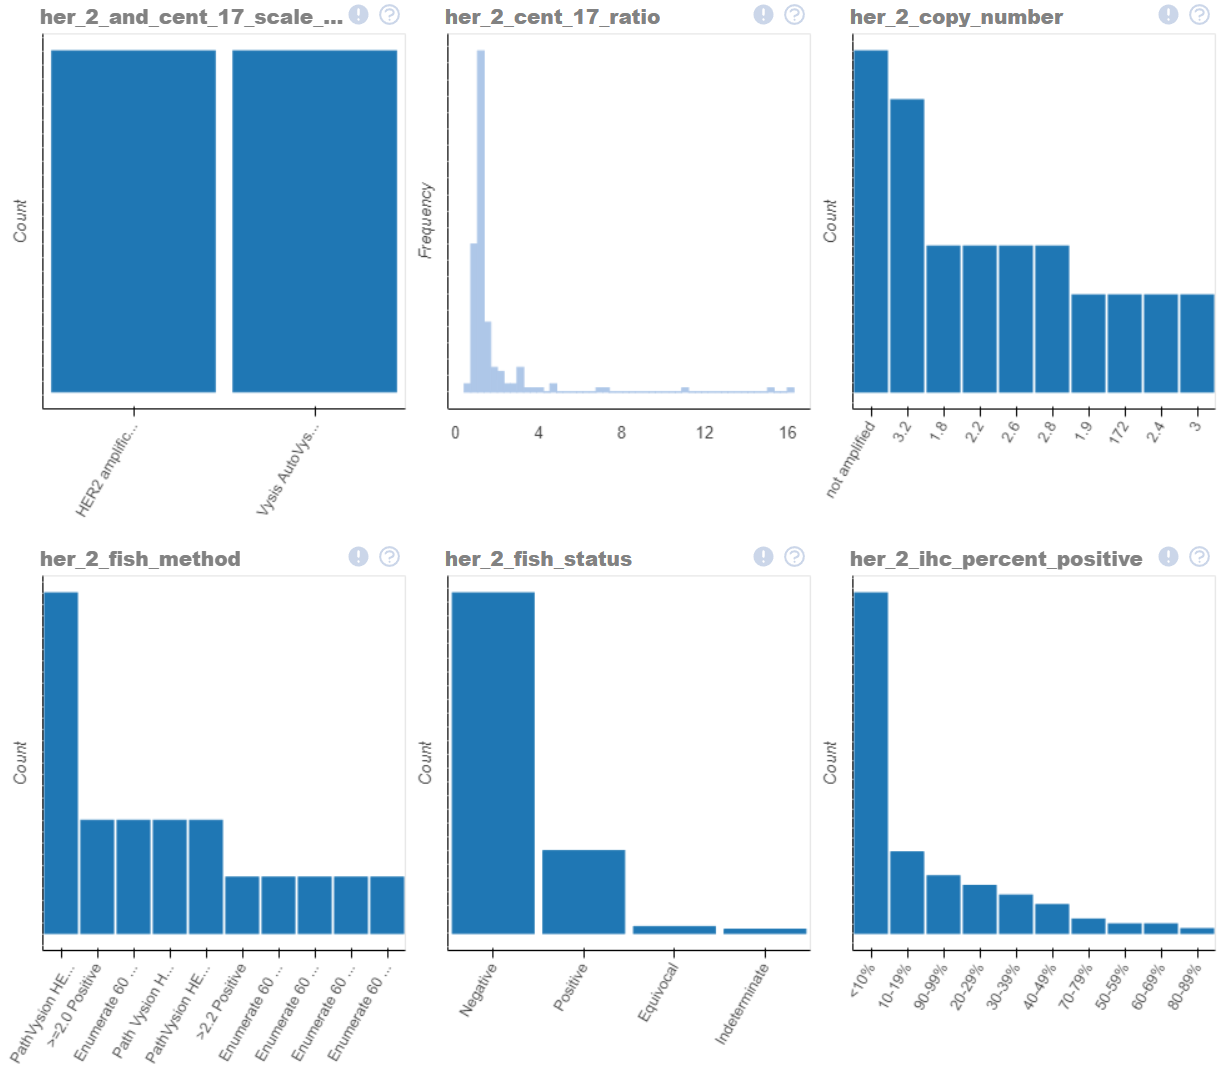
\includegraphics[width=0.9\textwidth]{NOTEBOOK/IMAGES_EDA/6}
\end{figure}

\begin{figure}
	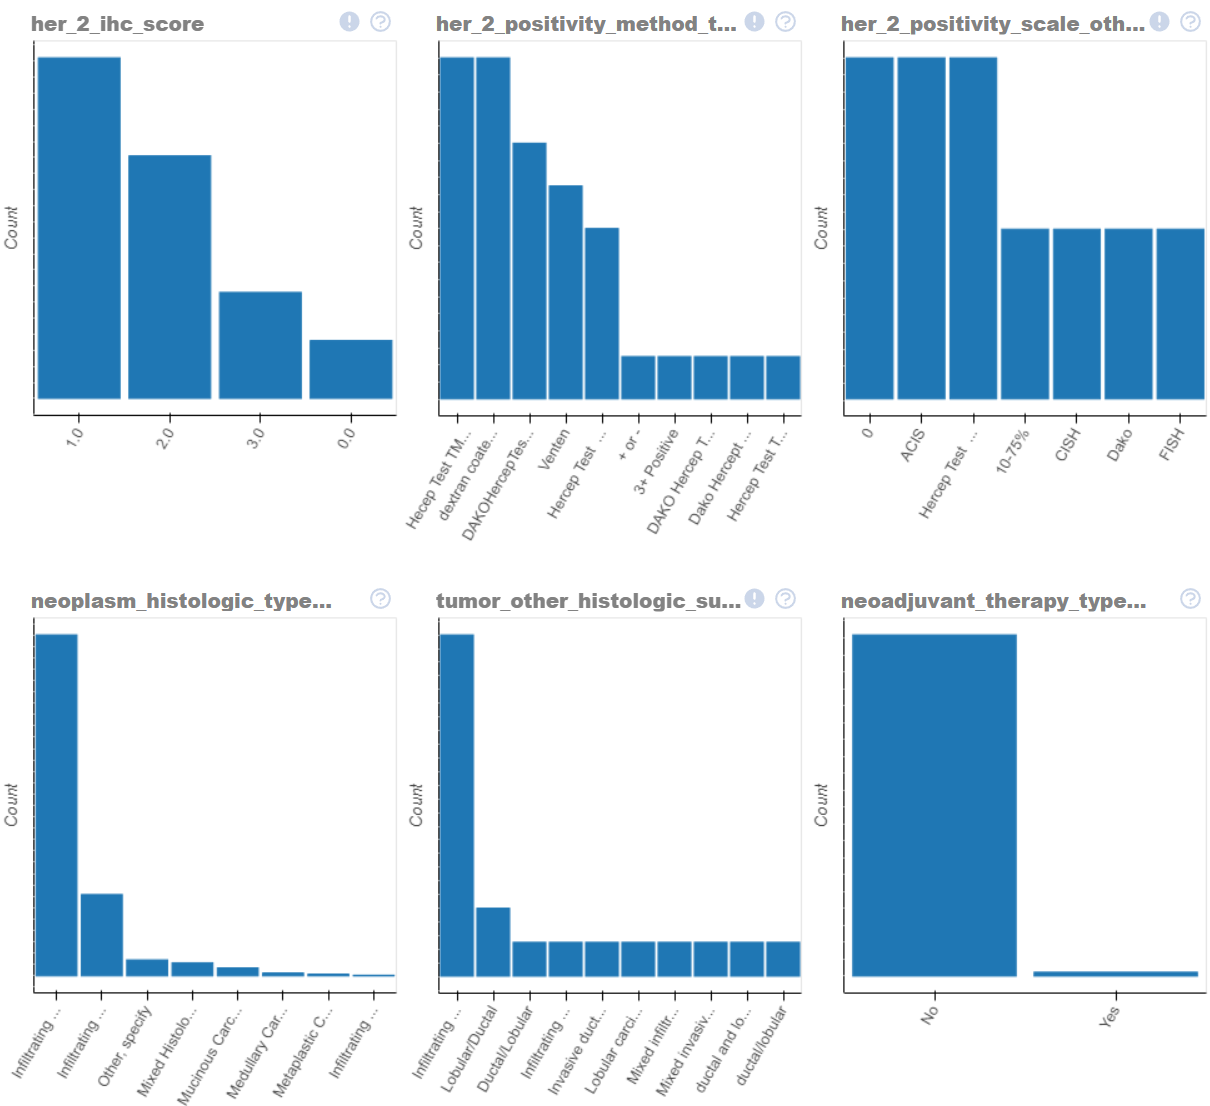
\includegraphics[width=0.9\textwidth]{NOTEBOOK/IMAGES_EDA/7}
	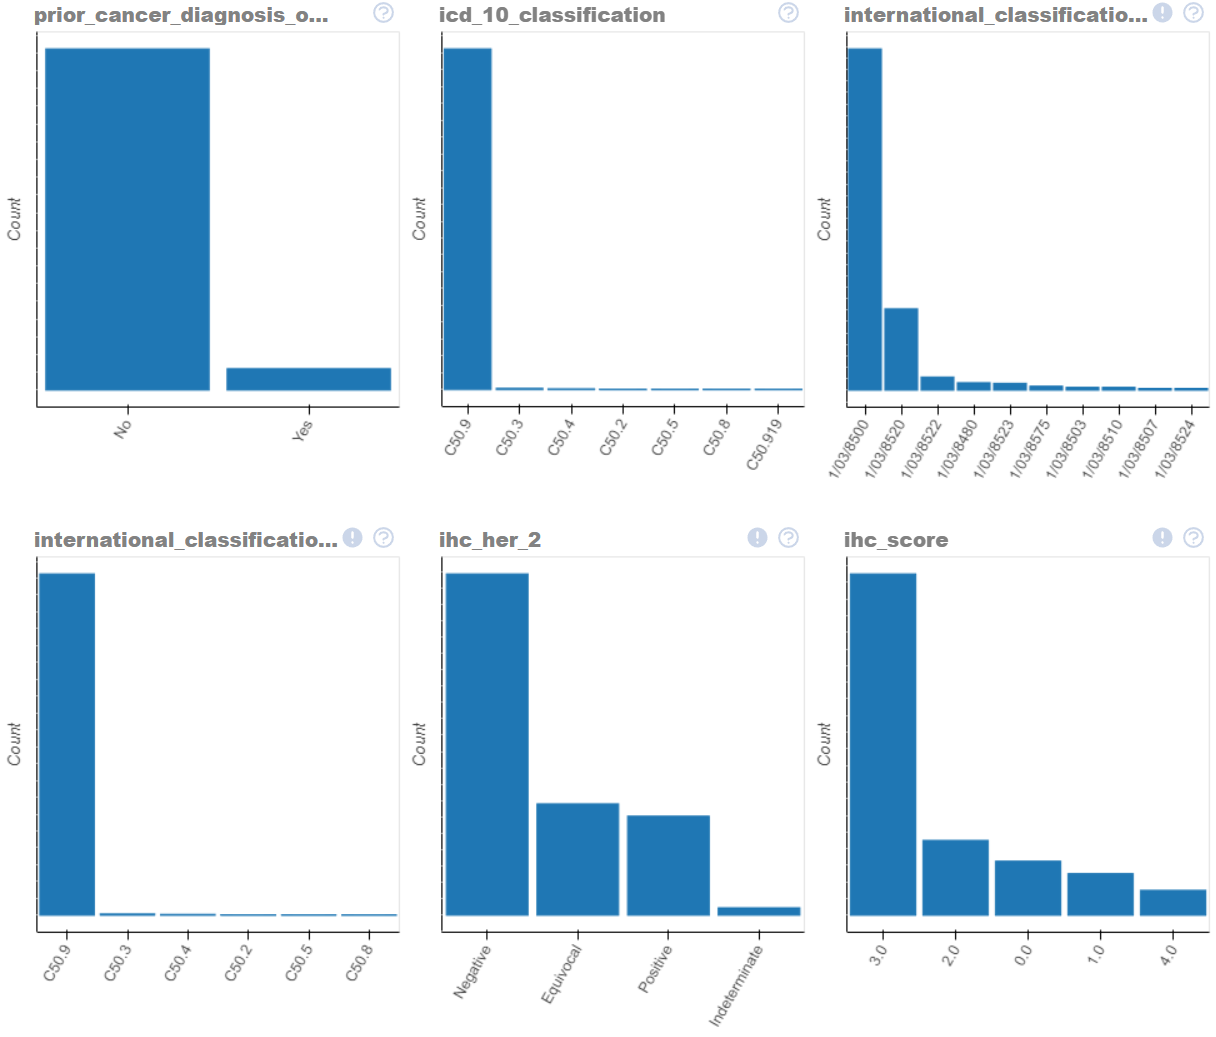
\includegraphics[width=0.9\textwidth]{NOTEBOOK/IMAGES_EDA/8}
\end{figure}

\begin{figure}
	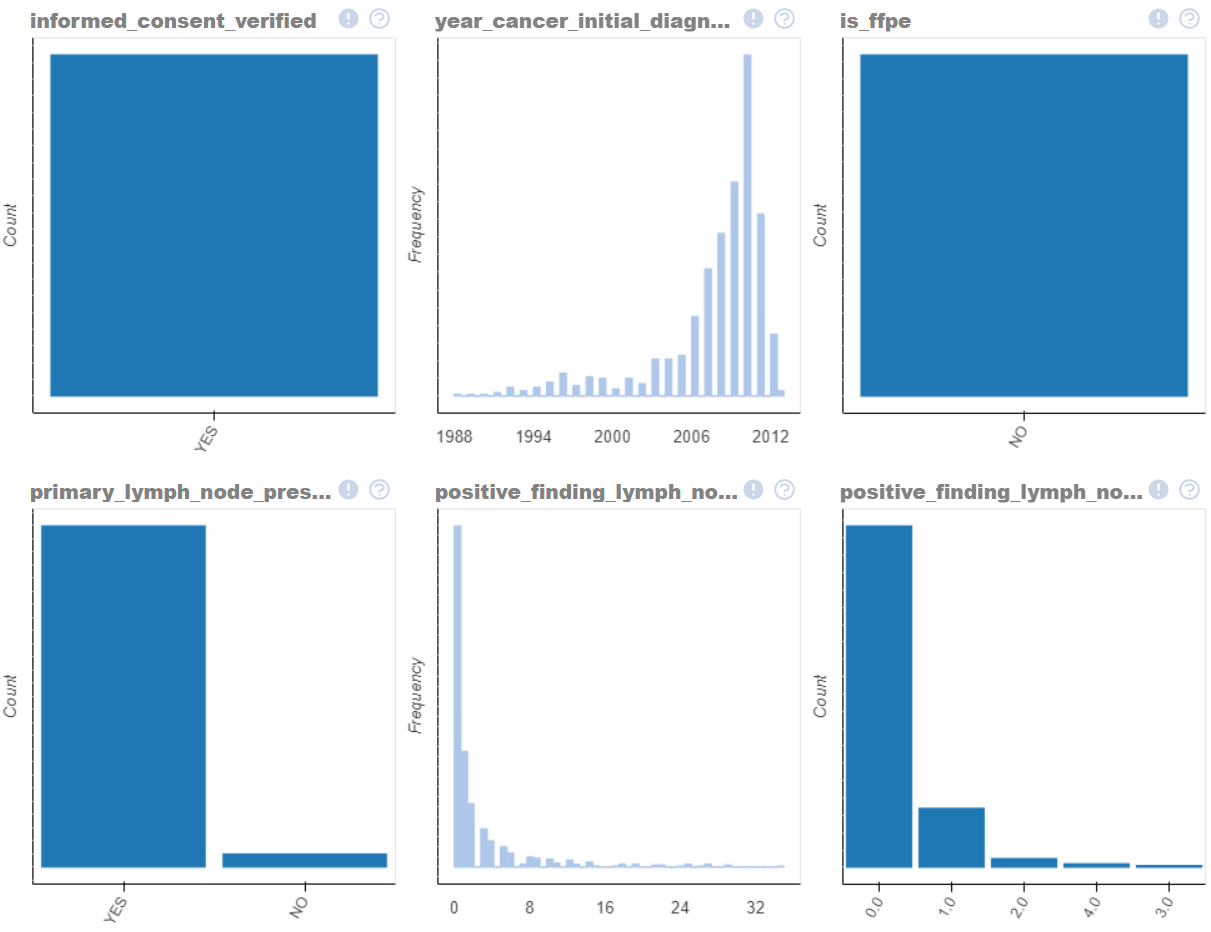
\includegraphics[width=0.9\textwidth]{NOTEBOOK/IMAGES_EDA/9}
	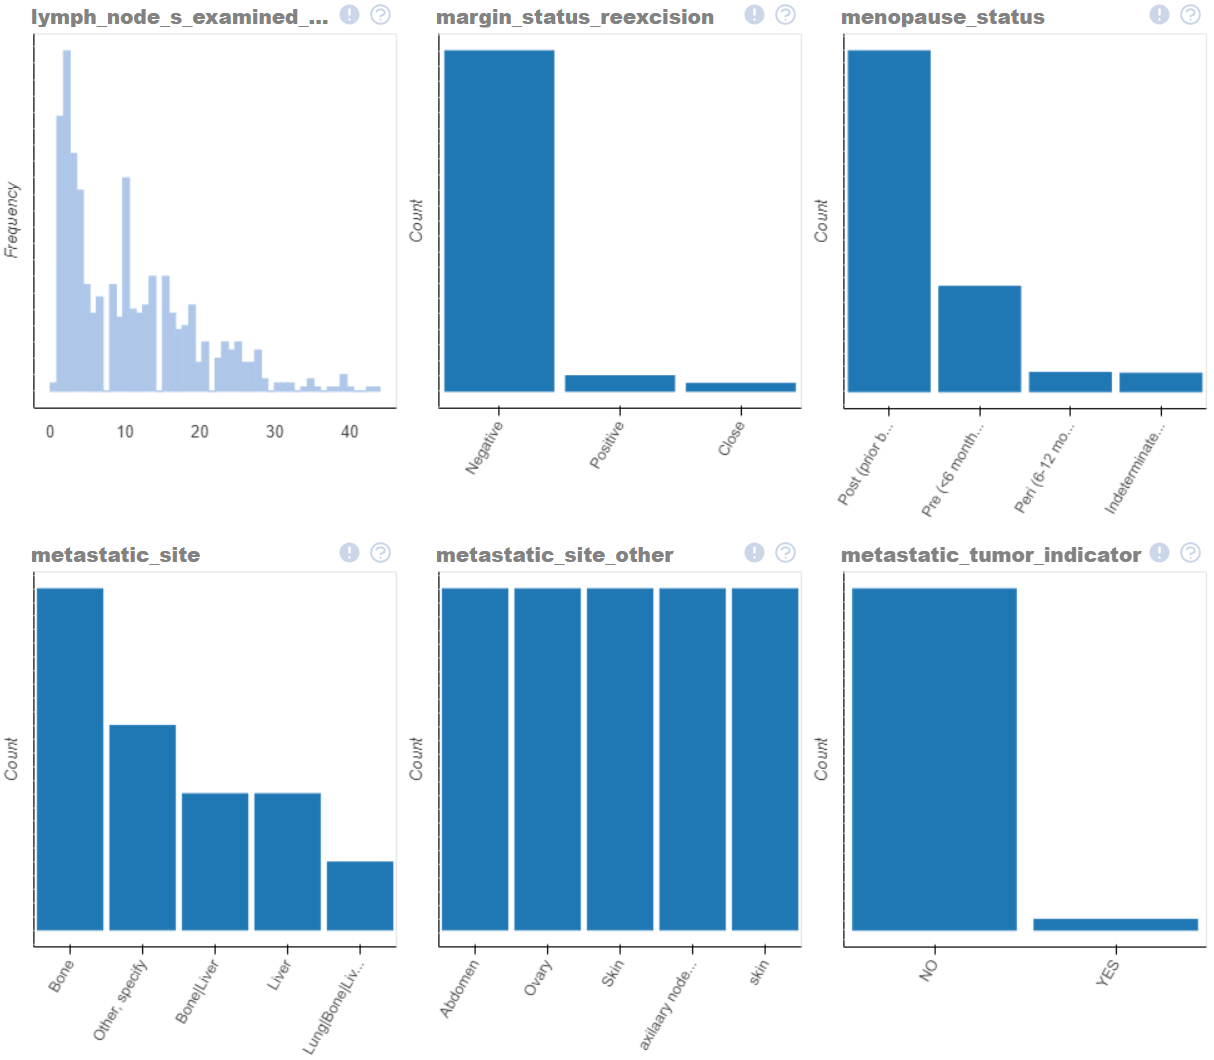
\includegraphics[width=0.9\textwidth]{NOTEBOOK/IMAGES_EDA/10}
\end{figure}

\begin{figure}
	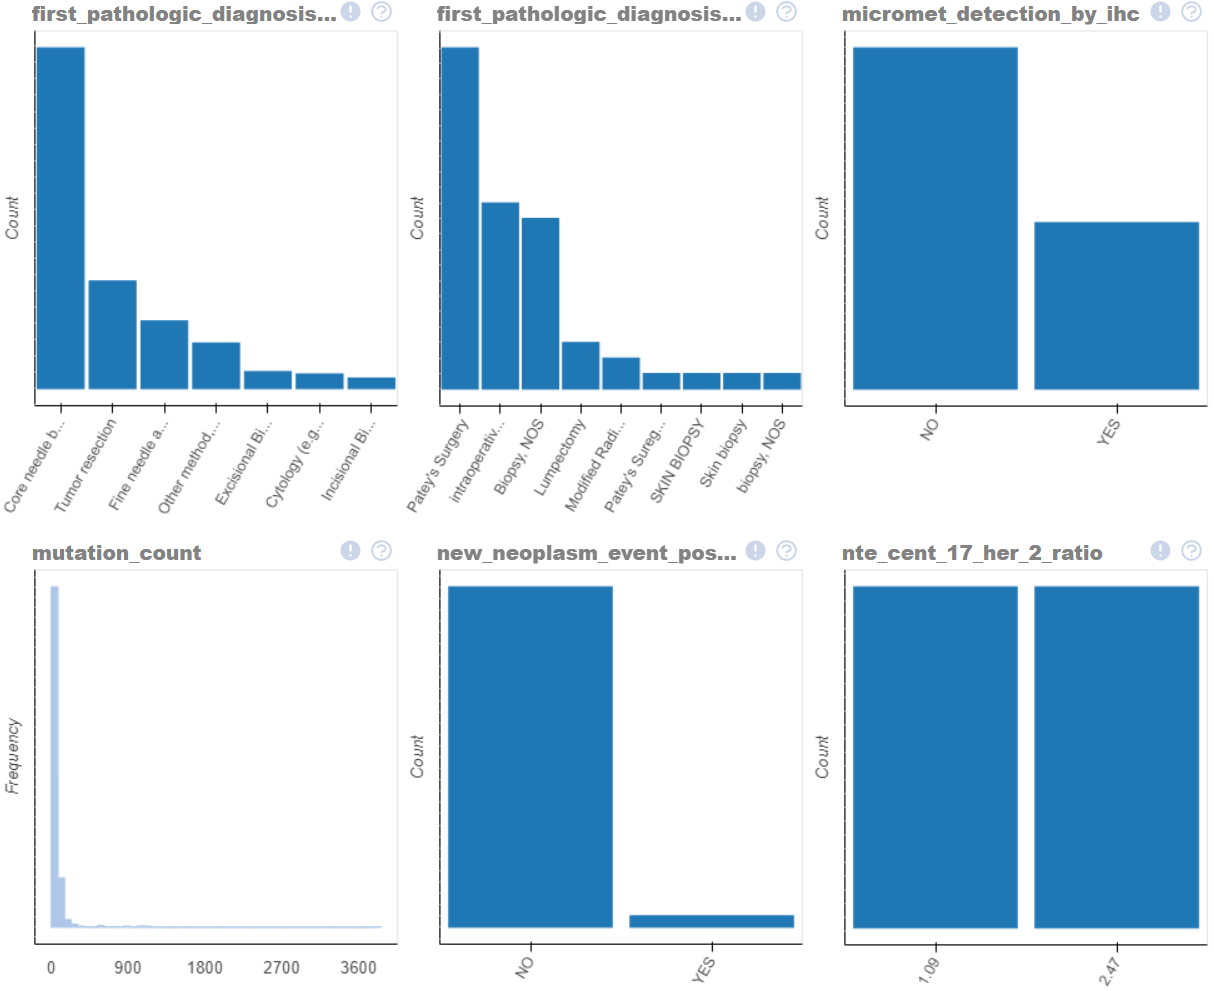
\includegraphics[width=0.9\textwidth]{NOTEBOOK/IMAGES_EDA/11}
	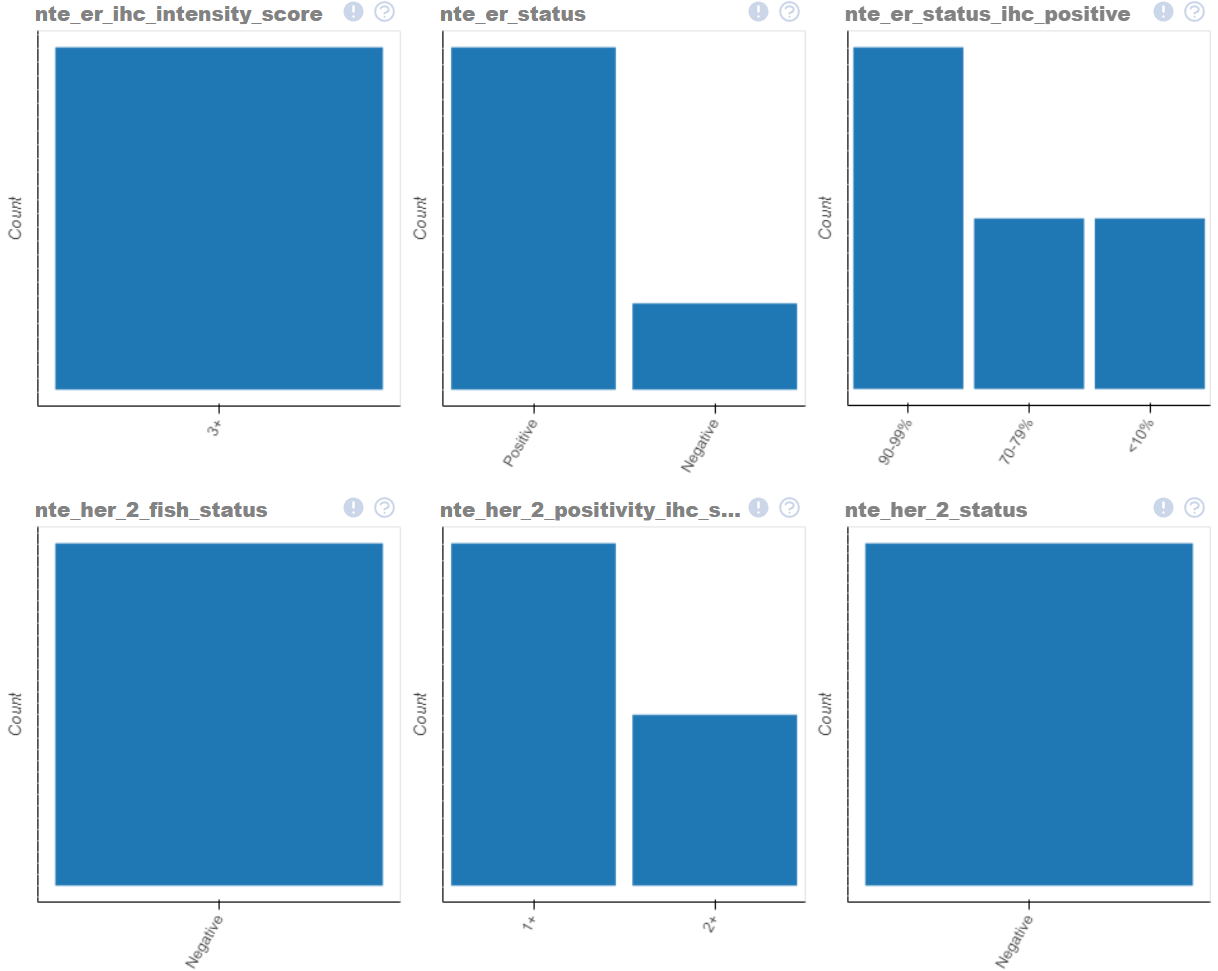
\includegraphics[width=0.9\textwidth]{NOTEBOOK/IMAGES_EDA/12}
\end{figure}

\begin{figure}
	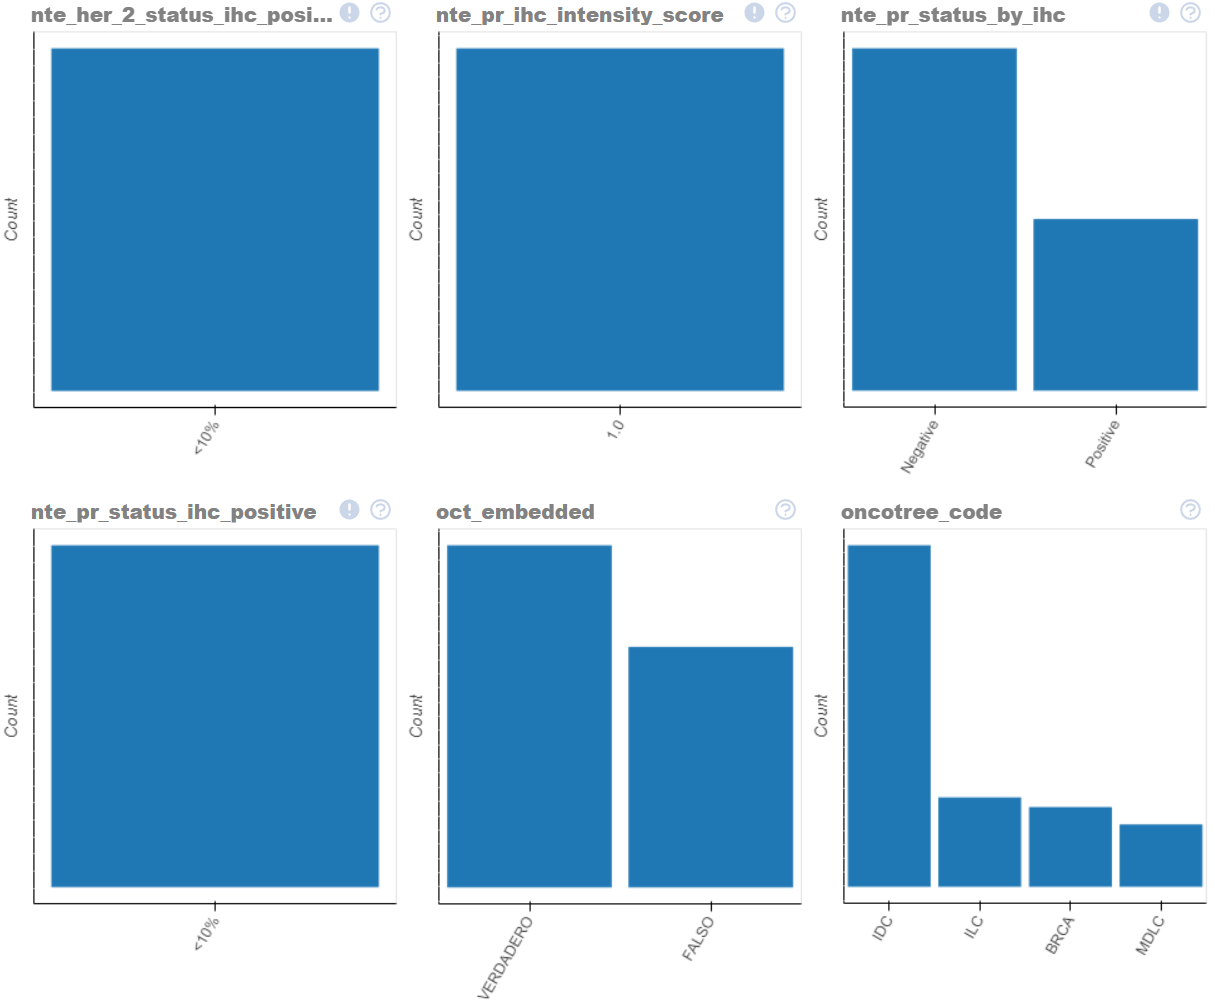
\includegraphics[width=0.9\textwidth]{NOTEBOOK/IMAGES_EDA/13}
	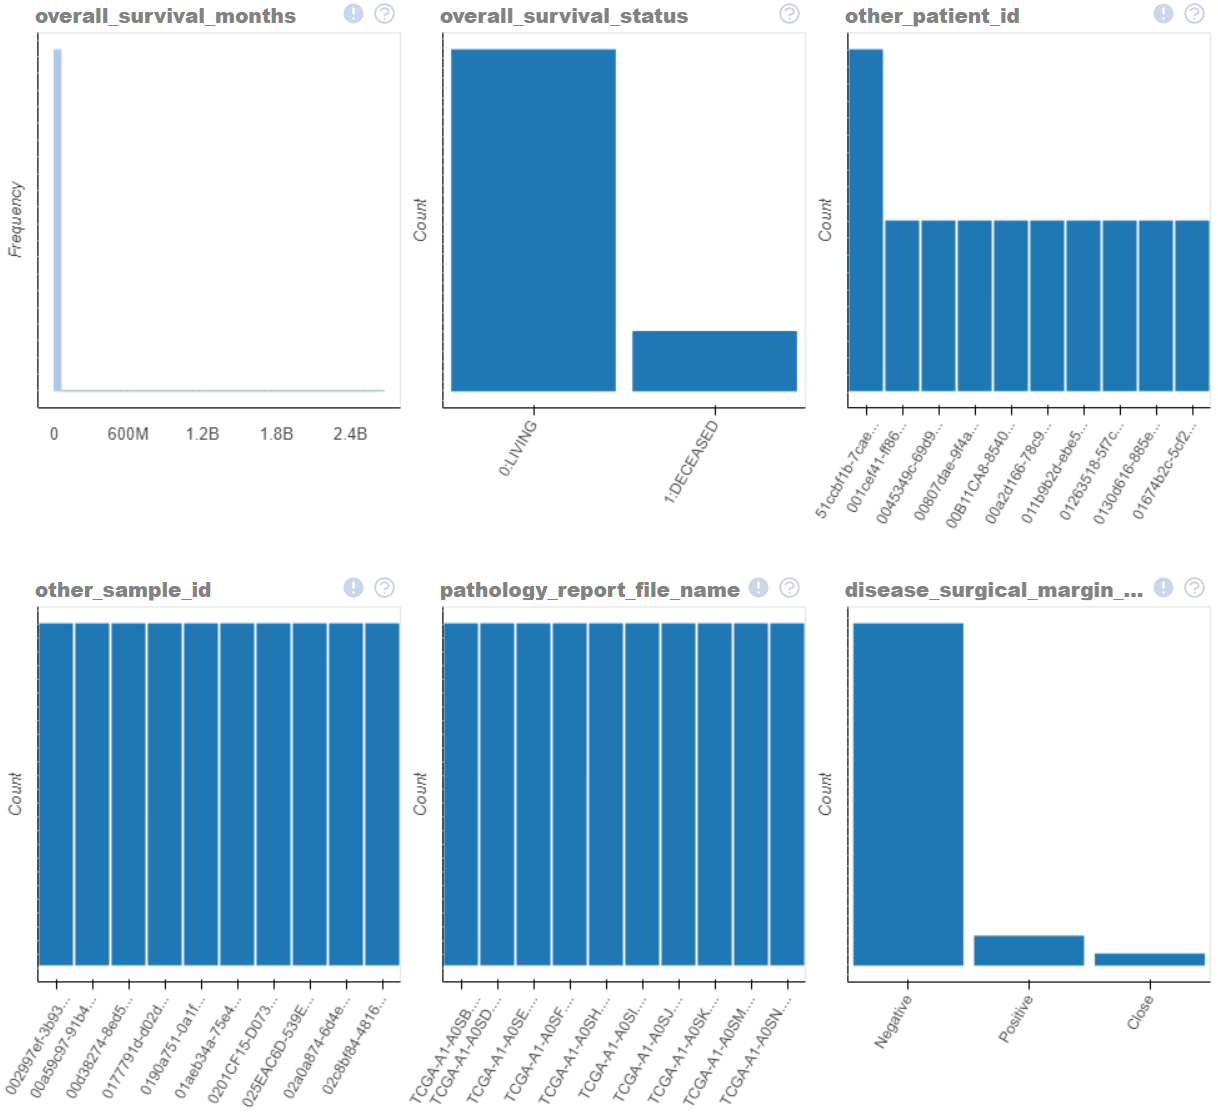
\includegraphics[width=0.9\textwidth]{NOTEBOOK/IMAGES_EDA/14}
\end{figure}

\begin{figure}
	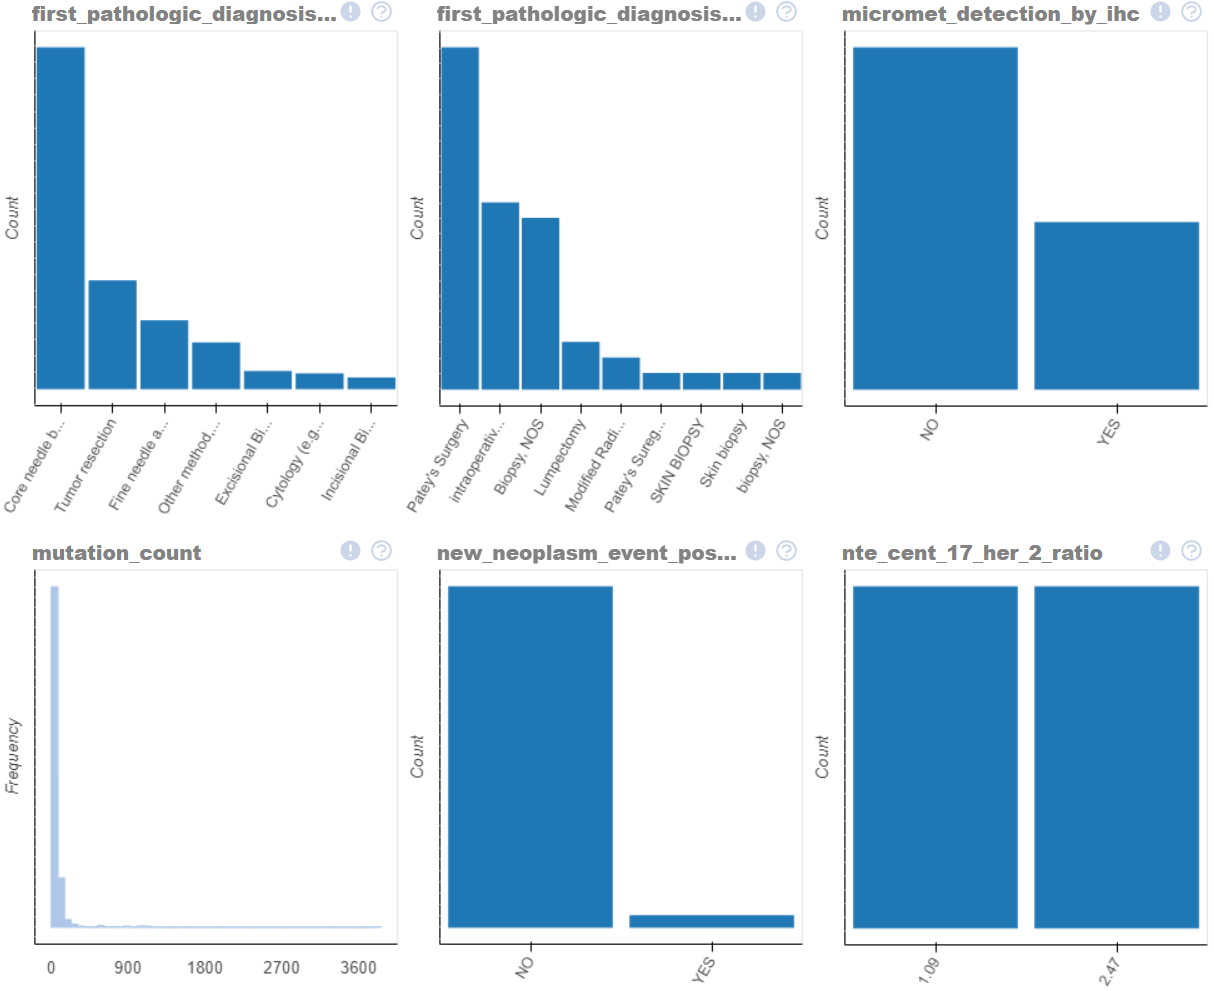
\includegraphics[width=0.9\textwidth]{NOTEBOOK/IMAGES_EDA/11}
	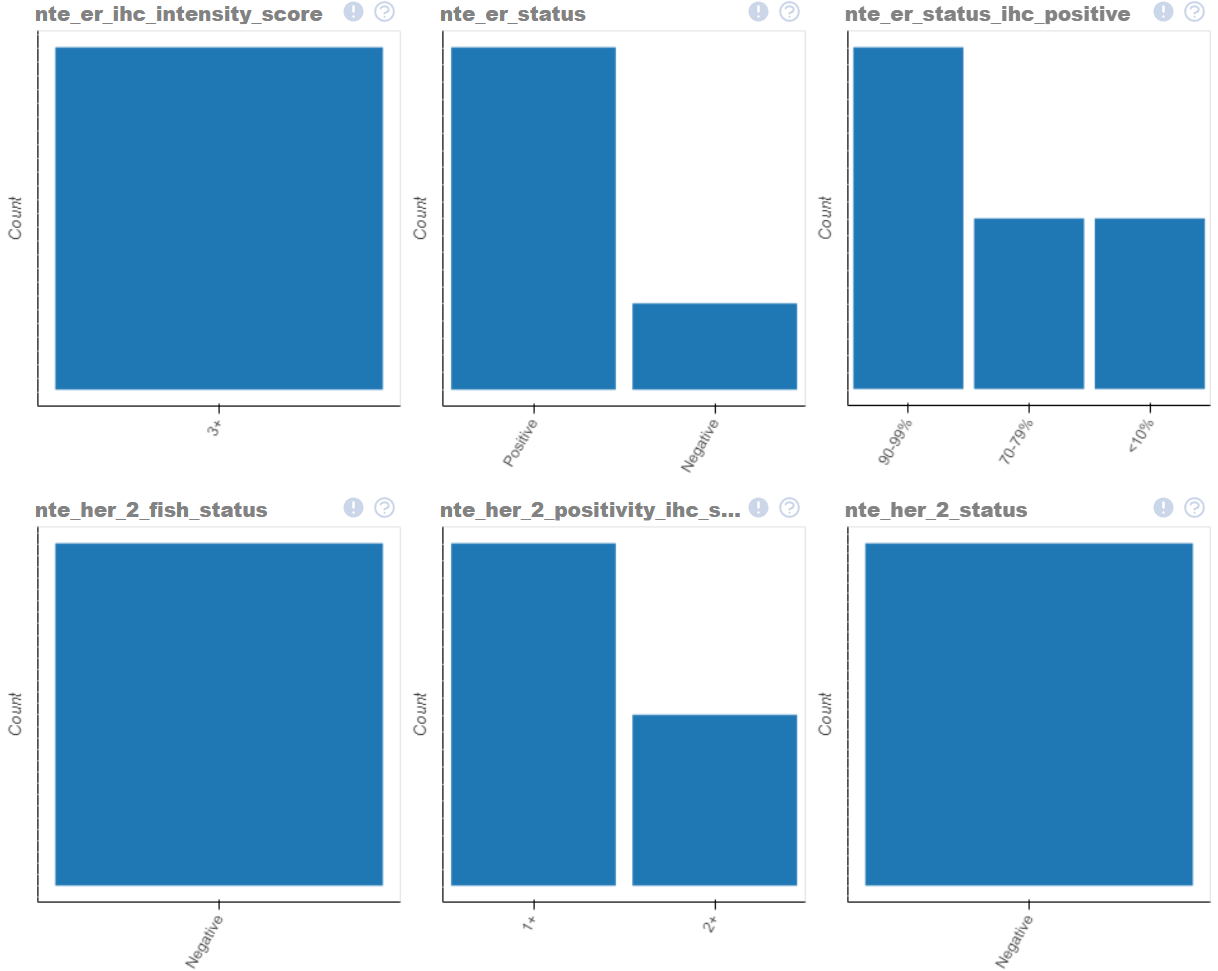
\includegraphics[width=0.9\textwidth]{NOTEBOOK/IMAGES_EDA/12}
\end{figure}

\begin{figure}
	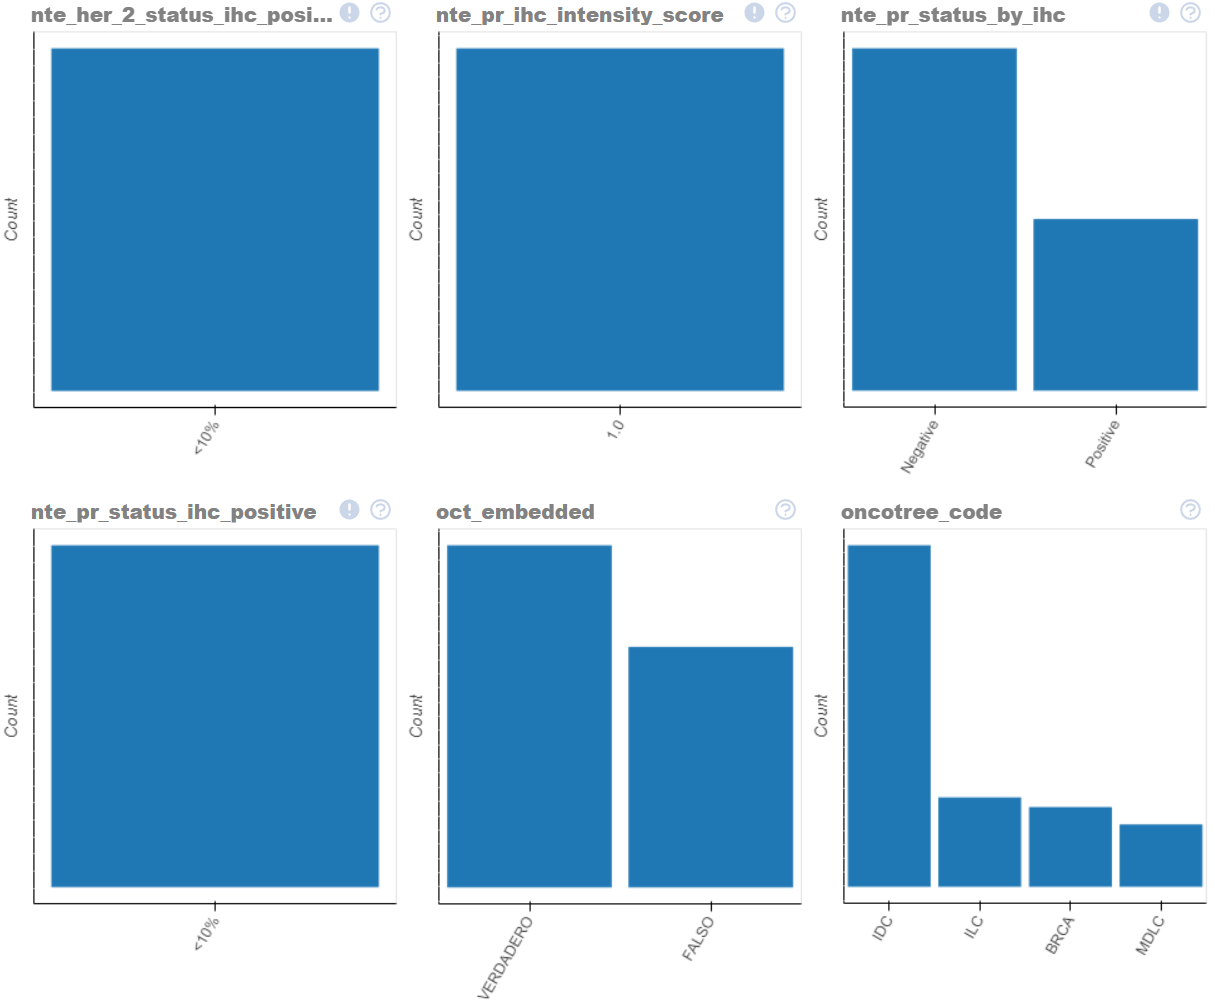
\includegraphics[width=0.9\textwidth]{NOTEBOOK/IMAGES_EDA/13}
	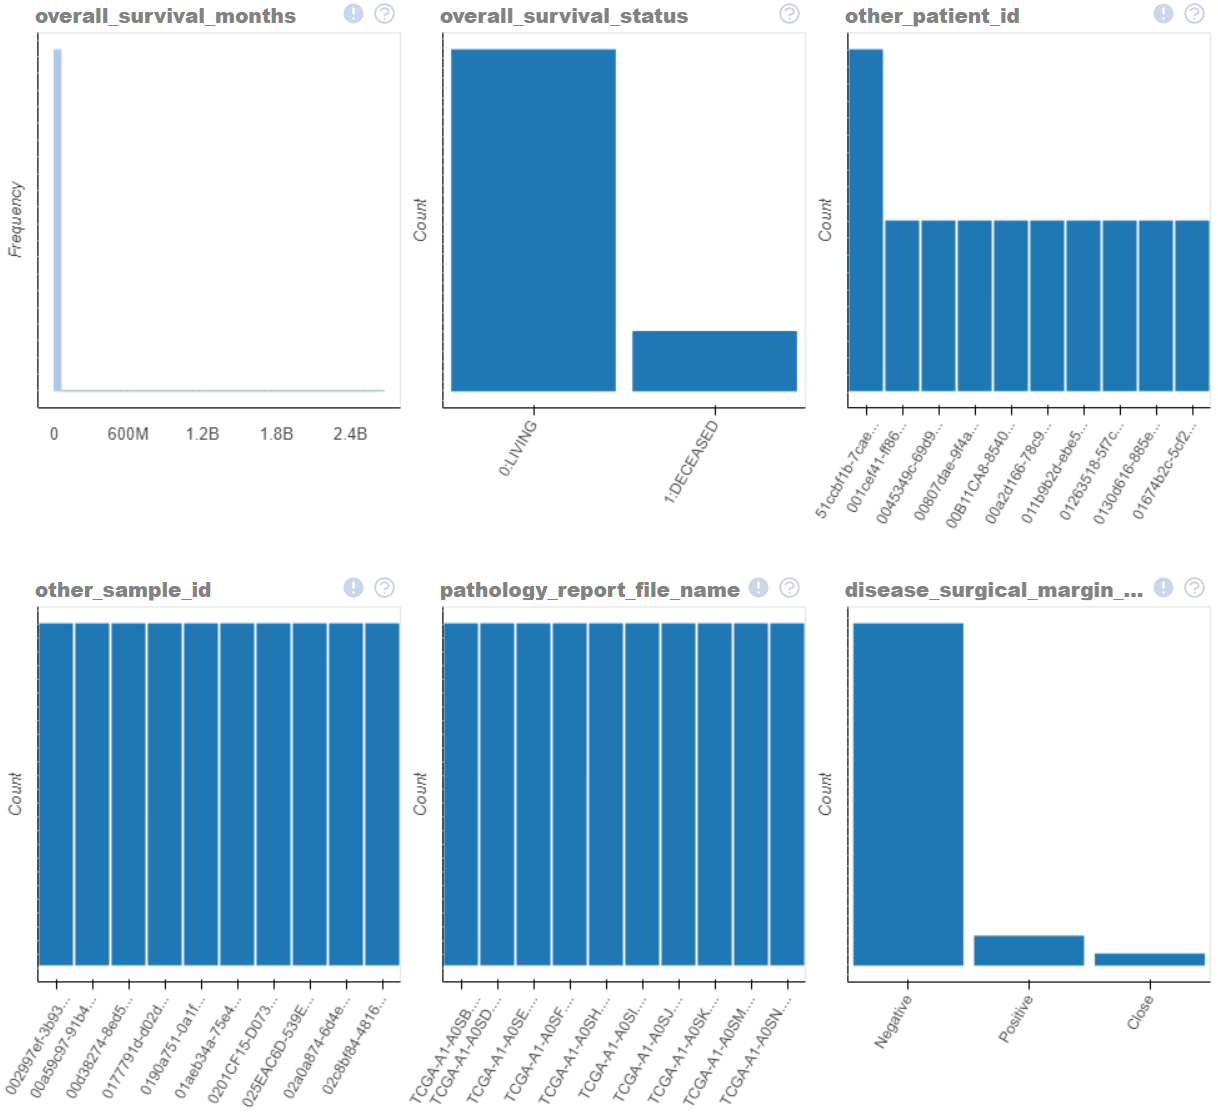
\includegraphics[width=0.9\textwidth]{NOTEBOOK/IMAGES_EDA/14}
\end{figure}

\begin{figure}
	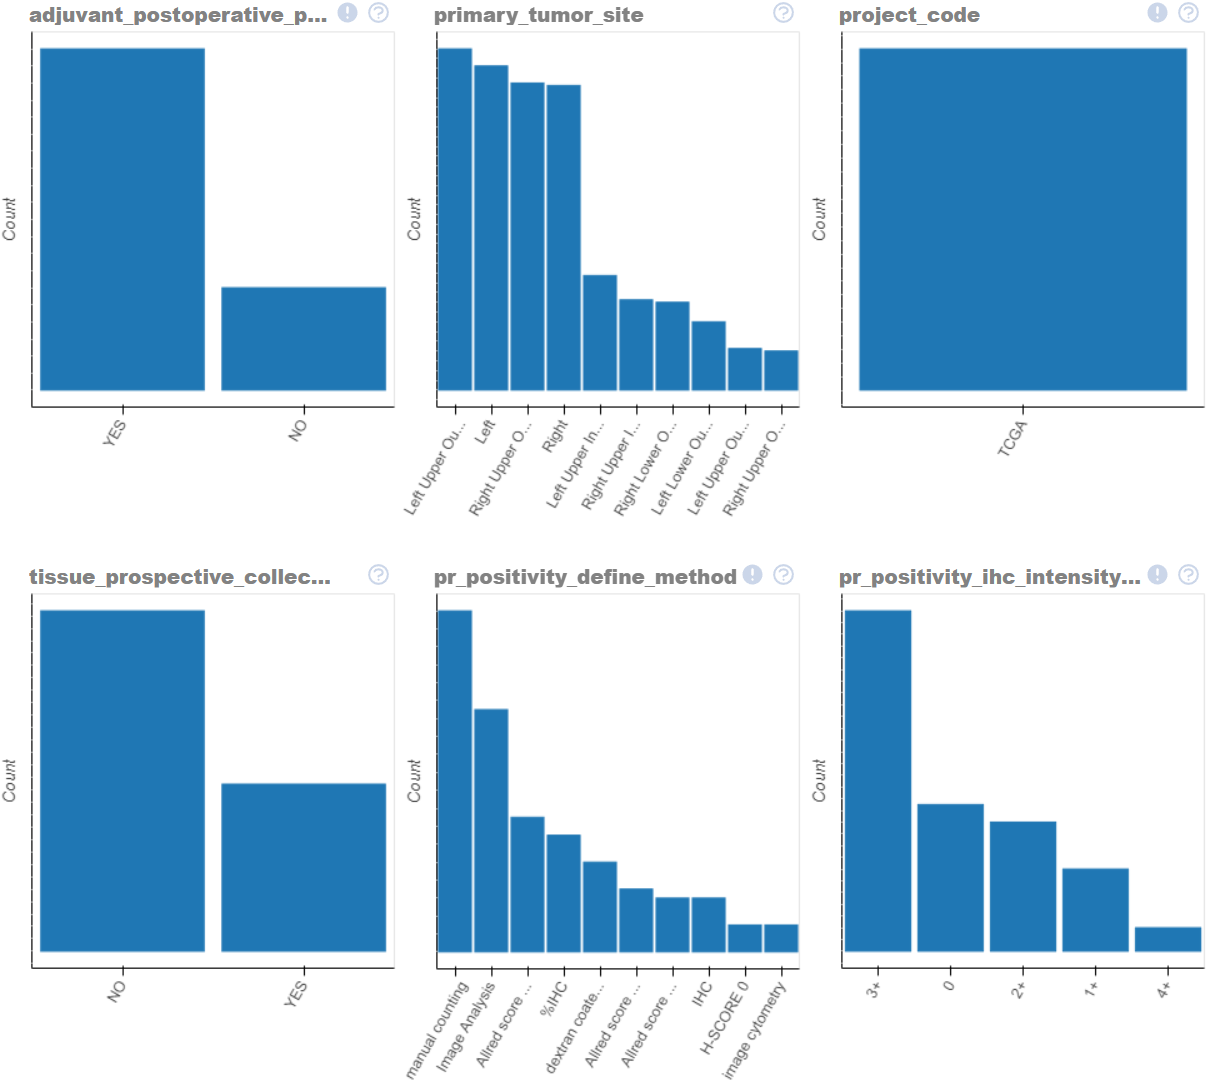
\includegraphics[width=0.9\textwidth]{NOTEBOOK/IMAGES_EDA/15}
	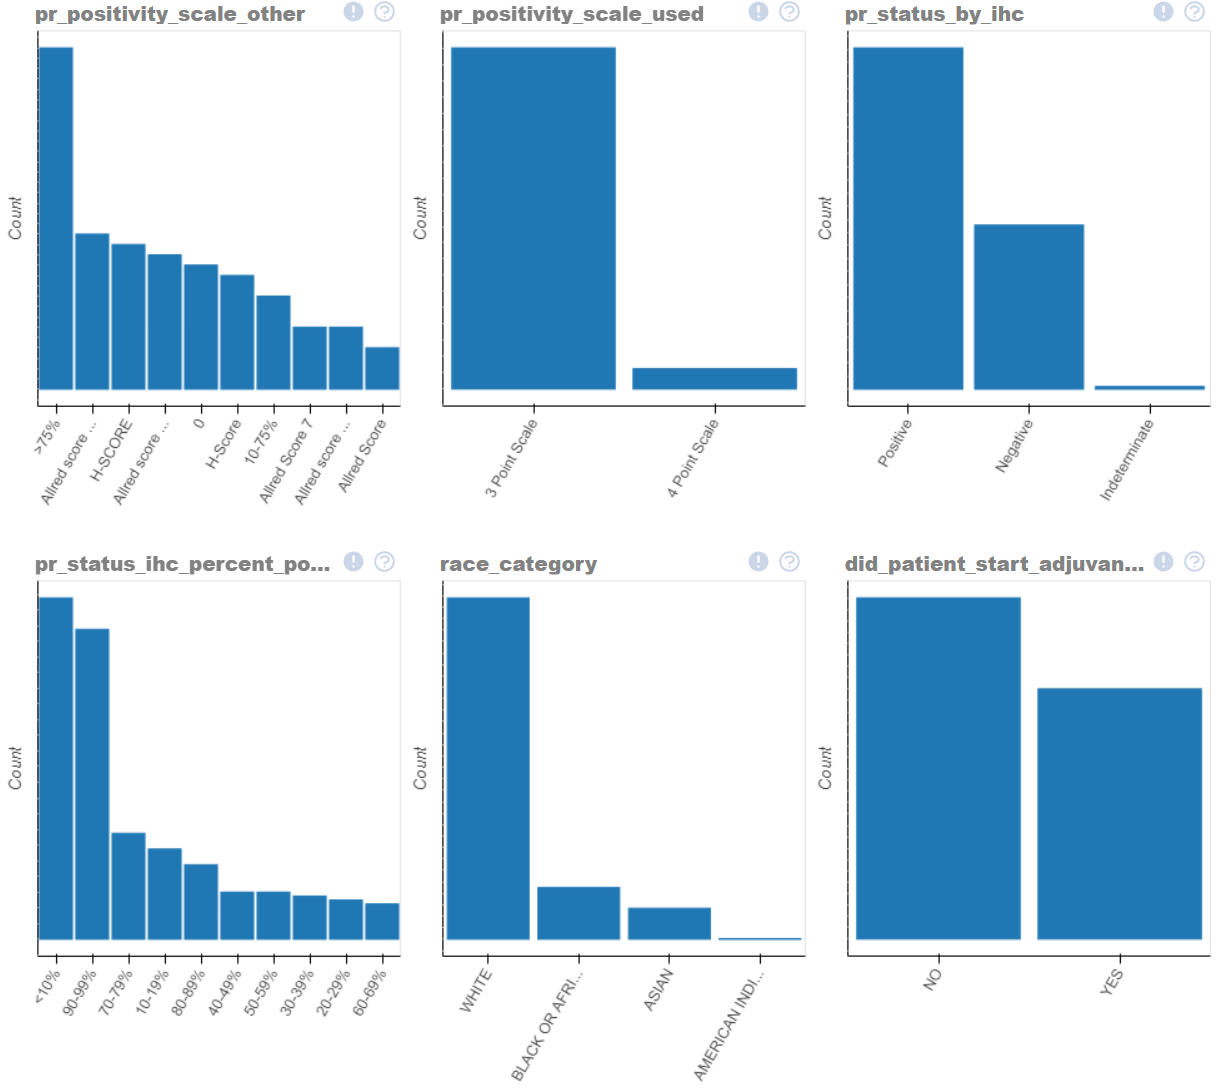
\includegraphics[width=0.9\textwidth]{NOTEBOOK/IMAGES_EDA/16}
\end{figure}

\begin{figure}
	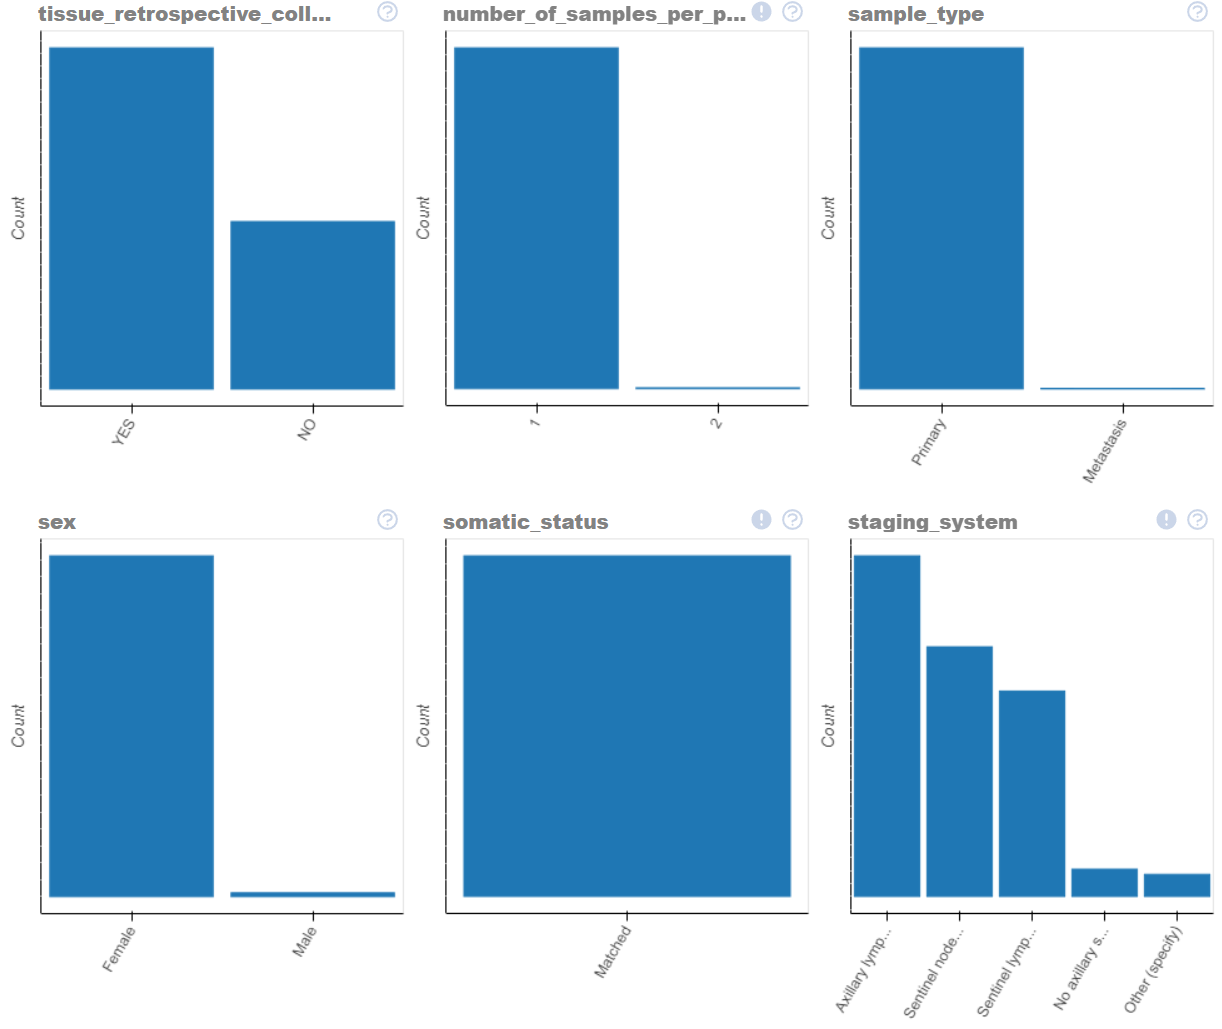
\includegraphics[width=0.9\textwidth]{NOTEBOOK/IMAGES_EDA/17}
	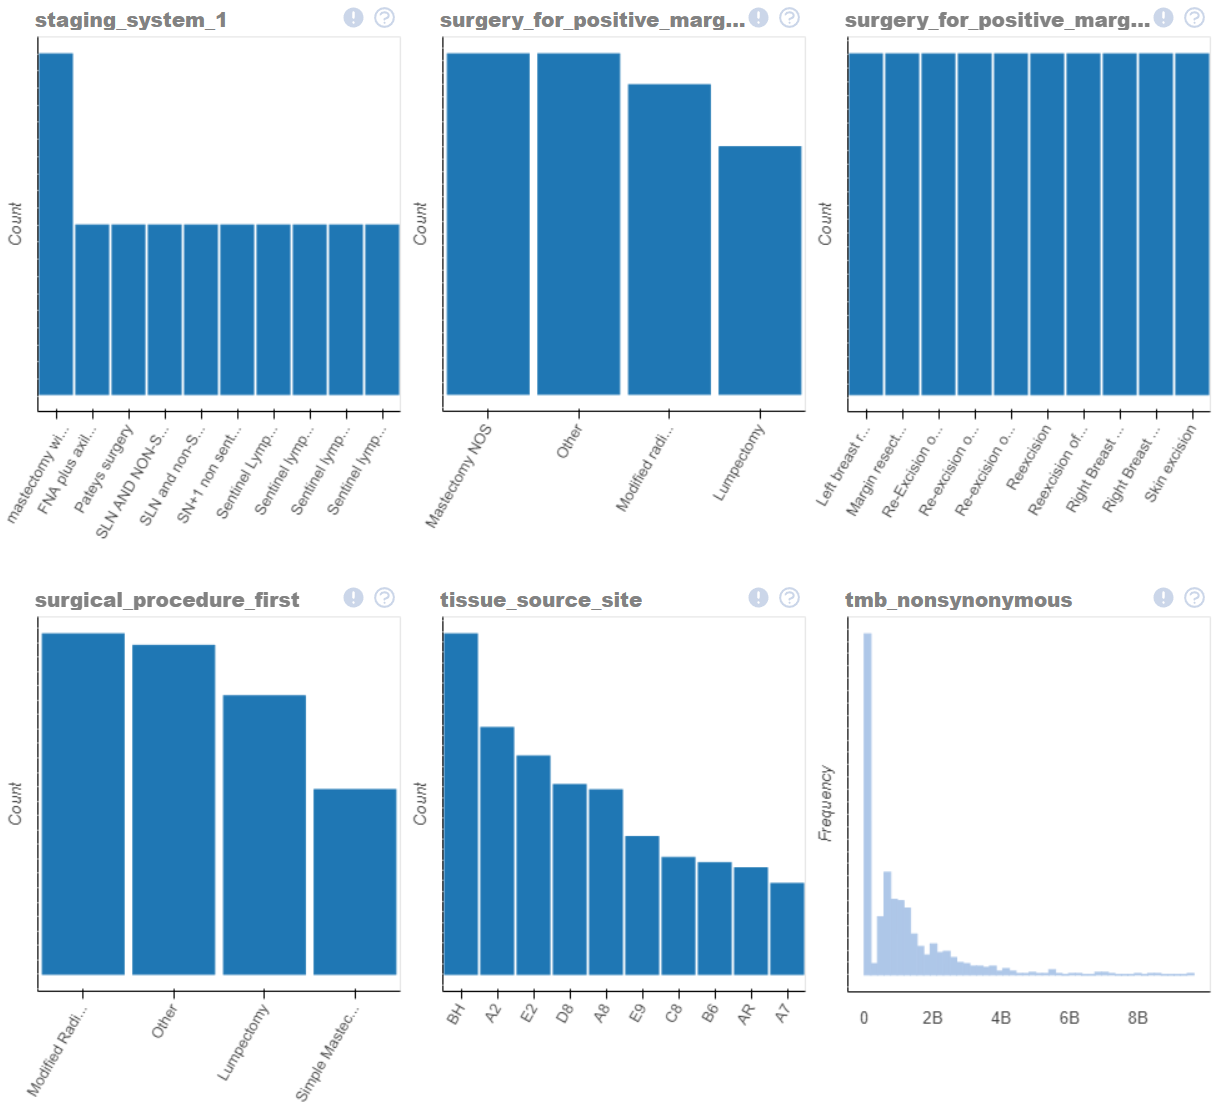
\includegraphics[width=0.9\textwidth]{NOTEBOOK/IMAGES_EDA/18}
\end{figure}

\begin{figure}
	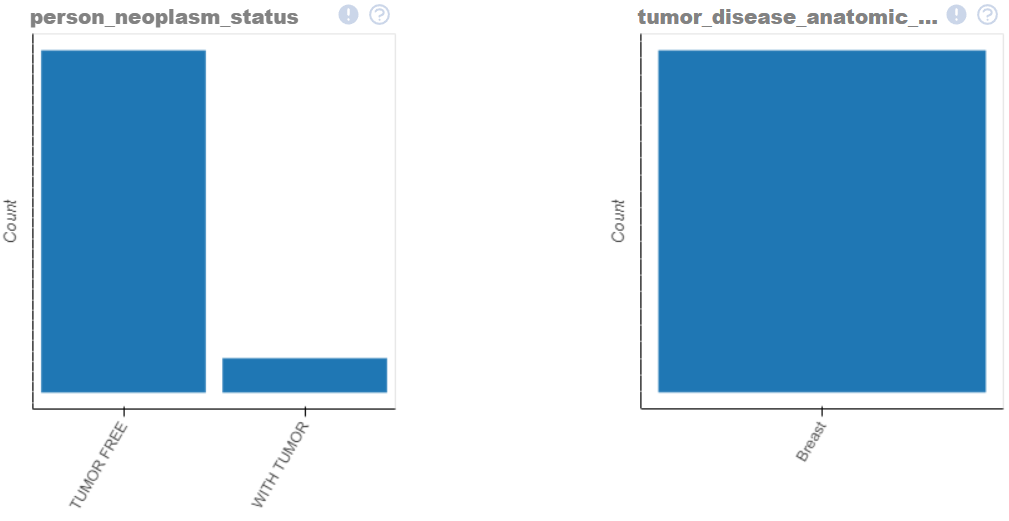
\includegraphics[width=0.9\textwidth]{NOTEBOOK/IMAGES_EDA/19}
\end{figure}